

\documentclass{beamer}
\usepackage{graphicx}
	\usetheme{CambridgeUs}

\begin{document}
\title{University of Dodoma\\ 
College of Informatics and Virtual Education\\
School of Informatics\\

\includegraphics[scale=0.5]{udomlogo}
}
\author{Mnyawami Yuda\\
HD/UDOM/127/T.2014\\
\textbf{MSc Information Technology}\\
\textbf{Name of Lecturer:} Mr. Faustine Antony
} 
\date{\today} 

\begin{frame}
\titlepage
\end{frame}
\begin{frame}
\frametitle{Wireless Communication and Applications}
\textbf{COGNITIVE RADIO}
\end{frame}

\begin{frame}
\frametitle{Outline:}
\begin{itemize}
\item Introduction in 5G\\
\item What drives 5G?\\
\item CR in 5G\\
\item Cognitive Cellular Networks \\
\item Future Research Directions\\
\item Conclusion\\
\end{itemize}
\end{frame}

\section{Introduction}
\begin{frame}
\frametitle{Introduction in 5G}
\begin{itemize}
\item Data Rates
\item Capacity
\item Spectrum
\item Energy
\item Latency
\item Reliability
\item Coverage
\item Devices per area
\end{itemize}
\end{frame}

\section{What drives 5G?}
\begin{frame}
\frametitle{What drives 5G?}

\textbf{Mobile data demand will continue to increase.}\\

Growth of existing applications.\\
\begin{itemize}
\item E-mail,\\ 
\item File transfer,\\ 
\item Real-time audio (VoIP),\\ 
\item Video streaming,\\
\item IP traffic,\\ 
\end{itemize}
\end{frame}

\begin{frame}
\frametitle{What drives 5G?}


\textbf{New applications and new ways of doing things
.}\\

\begin{itemize}
\item Instant Messaging (IM) with big files: lots of short connections, high data rates.\\
\item Internet-of-Things (IoT) and Machine-to-Machine (M2M): massive numbers of devices and connections, little data more than 50 billions of connected devices in 2020.\\
\item Critical applications - e.g., health, safety and security, traffic systems: guaranteed QoS.

\end{itemize}
\end{frame}

\section{Understanding of CR}
\begin{frame}
\frametitle{Meaning of Cognitive Radio}

It is an intelligent wireless communication system that is aware of its surrounding environment (i.e., outside world), and uses the methodology of understanding by building to learn from the environment and adapt its internal states to statistical variations in the incoming RF stimuli by making corresponding changes in certain operating parameters (e.g., transmit power, carrier frequency and modulation strategy) in real-time, with two primary objectives in mind: highly reliable communications whenever and wherever needed; and efficient utilization of the radio spectrum”.
\end{frame}

\section{Motivation}
\begin{frame}
\frametitle{The Motivation behind Cognitive Radio}
\textbf{Significant underutilization of the radio spectrum.}\\
\textbf{The Cognitive Radio solution to the spectrum underutilization problem:}
\begin{itemize}

\item Sense the radio environment to detect spectrum holes (i.e., underutilized subbands of the radio spectrum).
\item Make the spectrum holes available for employment by secondary users efficiently, subject to the constraint that the received power in each spectrum hole does not exceed a prescribed limit (set by the legacy user).

\end{itemize}
\end{frame}

\section{How it works}
\begin{frame}
\frametitle{How it works}
\textbf{The cognitive radio network is a complex multiuser wireless communication system capable of emergent behaviour.}\\
\textbf{It embodies the following functions:}
\begin{itemize}
\item To perceive the radio environment (i.e., outside world) by empowering each user’s receiver to sense the environment on a continuous-time basis;
\item To learn from the environment and adapt the performance of each transceiver (transmitter-receiver) to statistical variations in the incoming RF stimuli;
\end{itemize}
\end{frame}



\section{How it works}
\begin{frame}
\frametitle{How it works cont..}
\begin{itemize}
\item To facilitate communication between multiple users through cooperation in a self-organized manner;
\item To control the communication processes among competing users through the proper allocation of available resources;
\item To create the experience of intention and self-awareness.

\end{itemize}
\end{frame}

\section{Why may CR be interesting for 5G?}
\begin{frame}
\frametitle{Why may CR be interesting for 5G?}
\begin{itemize}
\item Some bands are significantly underutilized
\item Cost of dynamically leasing spectrum is expected to be much lower than purchasing a licensed band
\item Allows expansion of spectrum at a much lower cost
\item Coping with overload traffic
\end{itemize}
\end{frame}


\section{Cognitive cellular networks}
\begin{frame}
\frametitle{Cognitive cellular networks}
\textbf{Cognitive cellular networks}\\
Employs cognitive radio to lease addition spectrum outside the licensed cellular bands.\\

The radio resource(RR) at a particular band can be characterized
by;
\begin{itemize}
\item Bandwidth
\item Maximum transmit power
\item Reliability (or availability)
\end{itemize}
\end{frame}

\begin{frame}
\frametitle{Cognitive cellular networks}
\textbf{The RRs in a cognitive cellular network include;} 
\begin{itemize}
\item Licensed (cellular band) RR 
\item Cognitive RR
\end{itemize}

\textbf{Licensed radio resources (cellular bands)}
\begin{itemize}
\item Small bandwidth
\item High transmit power
\item High reliability
\end{itemize}
\textbf{Cognitive radio resources}
\begin{itemize}
\item Potentially broad bandwidth
\item Low transmit power
\item Low reliability
\end{itemize}
\end{frame}
\section{Architectures of Cognitive Cellular Networks}
\begin{frame}
It enables a cognitive cellular network to effectively integrate conventional licensed radio and cognitive radio into a holistic system. The architectures of cognitive cellular
networks can be categorized broadly into two types: non-cooperative and cooperative\end{frame}
\subsection{Non-Cooperative Architecture}
\begin{frame}
\frametitle{Non-Cooperative Architecture}
\begin{itemize}
\item From figure below, there are two separate radio interfaces operating at the licensed and cognitive RRs.
\item The cognitive RR is used to build a new network (i.e., a standalone cognitive network) that overlays the existing licensed cellular network.
\item Two separated networks at the physical layer
\item Integration at upper layers
\end{itemize}
\end{frame}
\begin{frame}
\frametitle{Non-Cooperative Architecture}
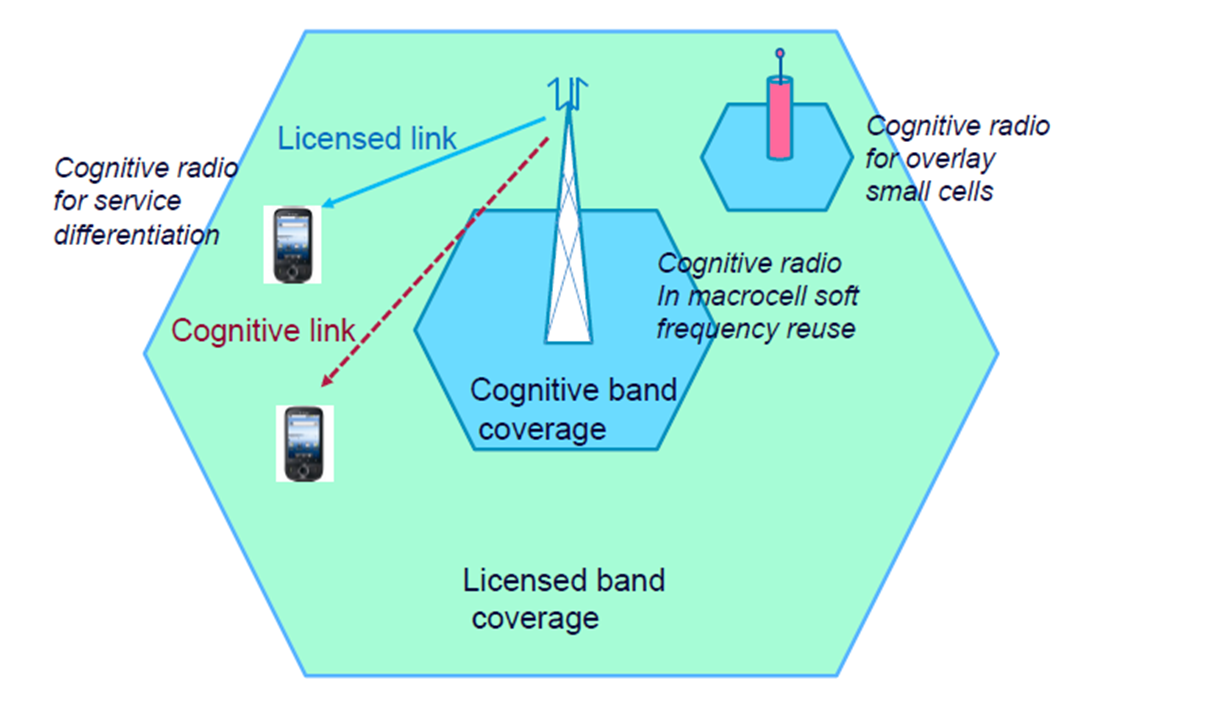
\includegraphics[scale=0.5]{nonartch}
\end{frame}
\section{Architectures of Cognitive Cellular Networks}
\subsection{Cooperative Architecture}
\begin{frame}
\frametitle{Cooperative Architecture}
\begin{itemize}

\item Combined used of licensed and CR resources to form a single integrated network
\item Using Cooperative communications allow distributed users to process and relay information in a coordinated fashion to achieve significant performance gains.
\end{itemize}
\end{frame}

\begin{frame}
\frametitle{Cooperative Architecture}
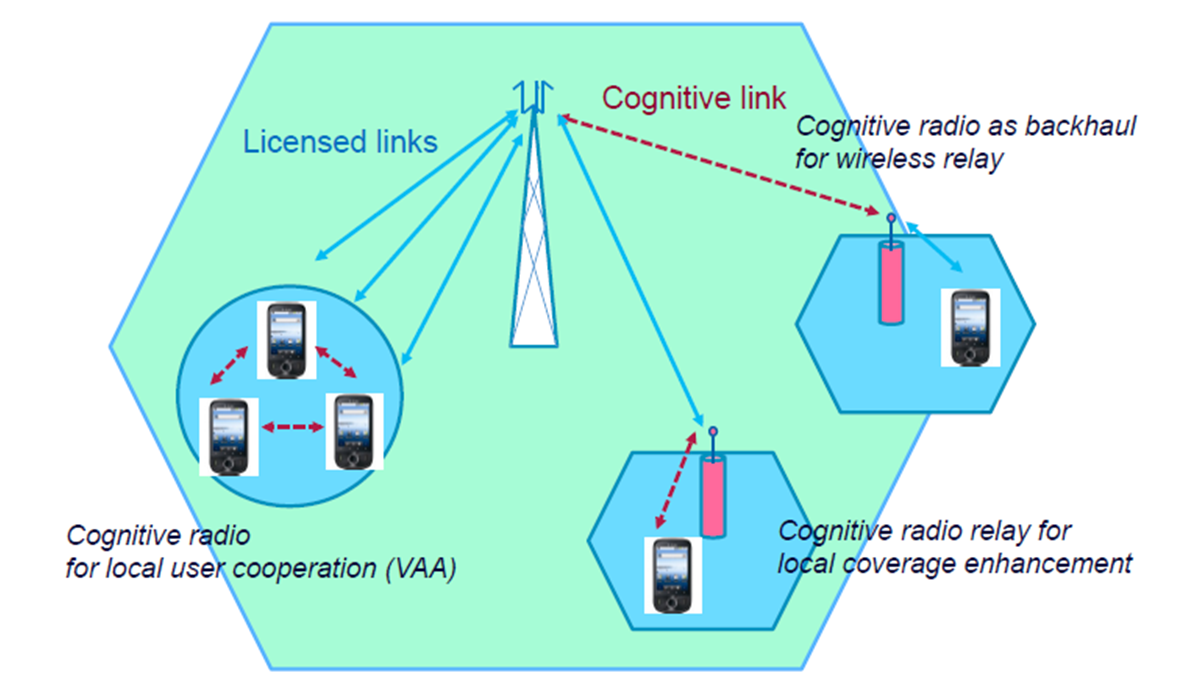
\includegraphics[scale=0.5]{arch}
\end{frame}

\begin{frame}
\frametitle{Major Functional Blocks of Cognitive Radio}
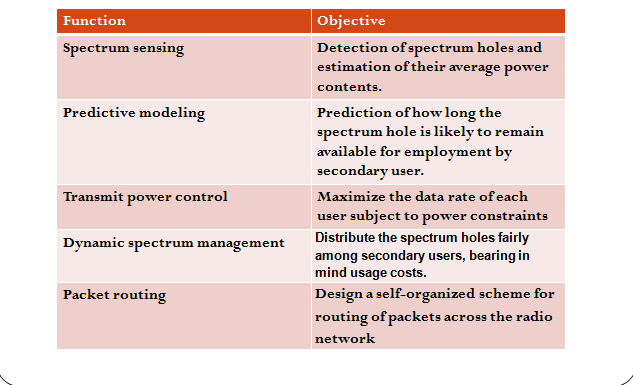
\includegraphics[scale=0.75]{fns}
\end{frame}

\section{Main in CR issues}
\begin{frame}
\frametitle{Main in CR issues}
\textbf{Self Coexistence}\\
\begin{itemize}
\item To avoid secondary users to harmfully interfere with primary users.\\ 
\end{itemize}
\textbf{Accurate sensing}\\
\begin{itemize}
\item Sensing aims to determine if a channel is idle or busy in terms of primary user activity.\\
 \end{itemize}
\textbf{Optimized spectrum decision}\\
\begin{itemize}
\item Secondary users are expected to dynamically choose the best available channels and transmission parameters.\\
\end{itemize} 
\textbf{Seamless spectrum handover}\\
\begin{itemize}
\item No latency should be noticed by users during mobility.
\end{itemize} 
\end{frame}

\section{Main in CR issues}
\begin{frame}
\frametitle{Main in CR issues cont..}
\textbf{Cross layer design}\\
\begin{itemize}
\item Spectrum sensing is restricted only to the PHY and MAC layers, spectrum management (e.g., spectrum handover, decision making and scheduling) can be related to all upper layers, which makes interaction and coordination between the different layers of the protocol stack necessary.\\ 
\end{itemize}
\textbf{Energy efficiency}\\
\begin{itemize}
\item Have limited communication and resource requirements, since most of the devices are battery powered. 
\end{itemize}


\end{frame}


\section{Future Research Directions}
\begin{frame}
\frametitle{Future Research Directions}
\begin{itemize}
\item Seamless spectrum handovers
\item Proactive spectrum selection and interference avoidance
\item Interdependency between the propagation characteristics of radio signals and the frequency band in usage Energy efficiency
\item Validation of CR protocols\\
\item Energy efficiency
\end{itemize}
\end{frame}
\section{Conclusion}
\frametitle{Conclusion}
\begin{frame}
\begin{itemize}
\item Better utilization of frequency band
\item Quick and easy information access
\item Better connectivity in mobility environment\\ 

\end{itemize}
\end{frame}


\end{document}

